\documentclass[main]{subfiles}

\begin{document}

\chapter{Long reads assembly tools state of the art}

\section{Pipeline with correction}

\subsubsection{\canu} \label{subsubsec:sota:canu}

\canu is based on \toolsname{Celera} \cite{celera_first, celera_second}, we can split the \canu pipeline in three step, correction, trimming, assembly, before each step \canu search overlap between reads.

\paragraph{Overlapping}

To avoid all versus all alignment \mhap try to estimate which read share a common part by estimate a Jaccard distance between the set of \kmers of two reads. The Jaccard distance, present in equation \ref{sota:equ:jaccard_dist} evaluate the distance between two set by divide the intersection of set by union of set.

\begin{equation}
J_{\delta}(A,B) = 1 - J(A,B) = 1 -  J(A,B) = 1 - \frac{|A \cap B|}{|A \cup B|}
\label{sota:equ:jaccard_dist}
\end{equation}

Enumerate all \kmers of each reads and compute intersection and union of each set take many times. \mhap select a subset of \kmers to represent the read and compute a mash distance \cite{mash_distance} see equation \ref{sota:equ:mash_dist_def} 

\begin{equation}
J(A,B) = \frac{|A \cap B|}{|A \cup B|} \approx \frac{|S(A \cup B) \cap S(A) \cap S(B)|}{|S(A \cup B)|}
\label{sota:equ:mash_dist_def}
\end{equation}

$S(A)$ is a \kmers set compose by $s$ first \kmers of set $A$. \citeauthor{mash_distance} evaluate the error between mash distance and jaccard distance was in $\mathcal{O}(\frac{1}{\sqrt{s}})$, by default in \mhap $s=512$ so the error was smaller than 0.05.

In \mhap order \kmer with a \texttt{tf-idf} score, see equation \ref{sota:equ:tf_idf_def}. The \texttt{tf-idf} score come for text search domain, try to say if this term is specific to this document. \texttt{tf} for term frequency indicate if the term was present many times in document, $n_{i,j}$ how many time the term $i$ was present in document $j$ divide by the number of term in document $j$. \texttt{idf} for inverse document frequency evaluate if the term was present in many document or just in some document, $|\mathcal{D}|$ the number of document in dataset divide by $|\{d_{j}:t_{i}\in d_{j}\}|$ the number of document where the term $i$ was present.

\begin{equation}
\mathrm{tf-idf_{i,j}} = \mathrm{tf_{i,j}} \cdot \mathrm{idf_{i}} = \frac{n_{i,j}}{\sum_{k}n_{k,j}} \cdot \log{\frac  {|\mathcal{D}|}{|\{d_{j}:t_{i}\in d_{j}\}|}}
\label{sota:equ:tf_idf_def}
\end{equation}

In \mhap term was \kmer and document was read, this technique permit to reduce the number of kmer in set and keep kmer specific to a read. If two read share specific kmer they probably share a common part.

If two reads have a small mash distance \mhap compare the position of each \kmer in reads to determinate the overlap position.

\paragraph{Correction}

In \canu correction was performed by a part of \toolsname{FALCON} \cite{falcon}, \toolsname{falcon\_sense}. In this section we didn't present in details how \toolsname{falcon\_sense} work but only the main idea.

Some correction tools as \toolsname{falcon\_sense} use a Partial Order Alignment (POA) (introduce in \cite{poa}) to perform long read correction. For each read \texttt{$R_1$} we recruit all read share an overlap with him, and perform an exact alignment with him. This alignment was use to build a POA graph, in POA graph each base was a node and a direct edge was create between two base if the first base was before the second one in an alignment. If an edge was present in two alignment her weight was increment. After all alignment was add in the POA graph, we search weighed path in this graph, and follow to reconstruct the corrected sequence. An example of POA graph construction was present in figure \ref{sota:fig:canu:correction}

\begin{figure}[ht]
    \centering
    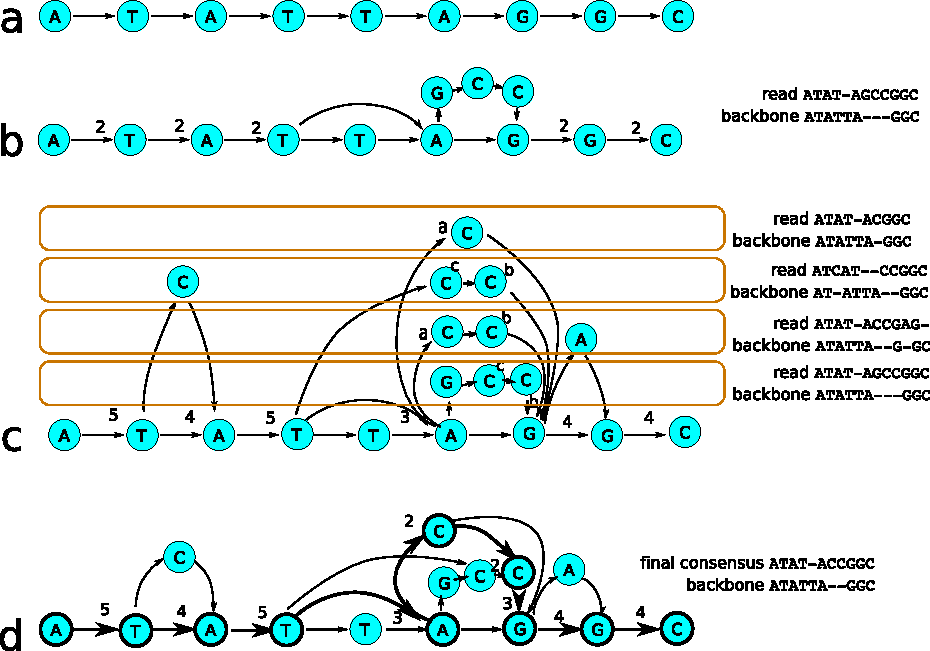
\includegraphics[width=\textwidth]{state_of_the_art/images/POA_explain.pdf}
    \caption{Sequence need to be correct was represent as a graph, each base was a node and if a base is follow by another an directed edge was build. (b) was the representation of sequence \texttt{ATATTAGGC} (call backbone in this figure), (b) We add the result of alignment of one read in the graph, number upper than edge was her weigth if and edge exist in some 3 alignment her weight was egal to 3, (c) We add all other alignment in the graph, (d) the bold path was choose a the correct path because it was supported by more alignment. This figure was originaly present in Supplementary material of \hgap \cite{hgap}}
    \label{sota:fig:canu:correction}
\end{figure}

\paragraph{Trimming}

The trimming step will remove the parts of the reads that are not supported by the other reads, see Figure \ref{sota:fig:canu:trimming}. For each reads we will analyze its coverage curve and remove the parts of the reads that are not sufficiently covered, for trimming \canu use an homemade tools.

\begin{figure}[ht]
    \centering
    \subfile{state_of_the_art/tikz/trimming.tex}
    \caption{Black line was a reads, the \canu trimming step keep only the blue part of read $R_0$, part covered by other read.}
    \label{sota:fig:canu:trimming}
\end{figure}

\paragraph{Assembly}

\canu assembly step is based on \OLC paradigm, with some specificity \canu build a Best Overlap Graph (BOG) for each not contained read only two overlap are kept in the graph, the best overlap for each read extremity, in \canu the best overlap was the longest overlap. After this graph construction step performed, some clean step was run, remove tips (a read with no sucessor), little buble.

This BOG was used as a scaffold to generate assembly, by remapping read against this scaffold, \canu try to detect repetition, larger than read not show in BOG as loop, and to call read to build a consensus after. Each simple path in BOG was used to build a contig. 


\subsection{Pipeline without correction}

\subsubsection{\miniasm} \label{subsubsec:sota:miniasm}

\miniasm \minimap was an assembly pipeline proposed in \cite{miniasm_minimap} and \cite{minimap2}, the main purpose of this pipeline is to demonstrate we can perform a long read assembly without correct long read.

\paragraph{\minimap}

\paragraph{\miniasm}

\subsubsection{\hinge}

\subsubsection{\wtdbg}

Use a \DBG approch to solve long-read assembly, isn't realy a \DBG but a "Fuzzy-Brujin graph" (\abreviation{FDBG}). To build this graph \wtdbg split read in bin with a fixed size (256 base pairs) and they store kmer present in each bin in a hash table.
To find overlap between reads wtdg2 use an hash table to compare the kmer composition between each reads and perform an exact alignment between each bin of reads. 

After this alignment step \wtdbg keep only in memory wich bin are align to which bin, and they build a k-bins each k-bins is a sequence of k successive bin in a read, \wtdbg can infer if two k-bins overlap if some bin in this two k-bins share an ovelap.

A group of K-bins are a node of \abreviation{FDBG}, \wtdbg build an edge between two node if a K-bins in each node are succesive in a read, after some cleanning step (pops bubbles, tips cleanning, etc…) \wtdbg build a consensus sequence with each simple path in \abreviation{FDBG}.

\onlyinsubfile{
\bibliographystyle{plainnat}
\bibliography{state_of_the_art}
\addcontentsline{toc}{chapter}{Bibliography}
}

\end{document}